\documentclass[12pt, twoside]{article}
\usepackage[francais]{babel}
\usepackage[T1]{fontenc}
\usepackage[latin1]{inputenc}
\usepackage[left=3mm, right=3mm, top=3mm, bottom=3mm]{geometry}
\usepackage{float}
\usepackage{graphicx} 
\usepackage{array}
\usepackage{multirow}
\usepackage{amsmath,amssymb,mathrsfs}
\usepackage{soul}
\usepackage{textcomp}
\usepackage{eurosym}
 \usepackage{variations}
\usepackage{tabvar}


\pagestyle{empty}

\begin{document}


\section*{\center{Devoir maison 6}}

\textit{Devoir � rendre sur feuille grand format petits
carreaux pour le \ul{jeudi 14 avril 2011}.}

\enskip


\textit{Remarque: La r�daction et la justifcation des r�sultats seront pris en
compte (et ont autant d'importance que les calculs).}

\subsection*{Exercice 1}

\begin{enumerate}
  \item VAR est un triangle rectangle en A tel que VA=15cm et VR=17cm. Calculer
  la longueur AR. 
  \item POT est un triangle rectangle en O tel que PO=120m et TO=119m. Calculer
  la longueur TP.
\end{enumerate}



\subsection*{Exercice 2}

Les triangles suivants sont-ils rectangles? Justifier votre r�ponse.

\begin{center}
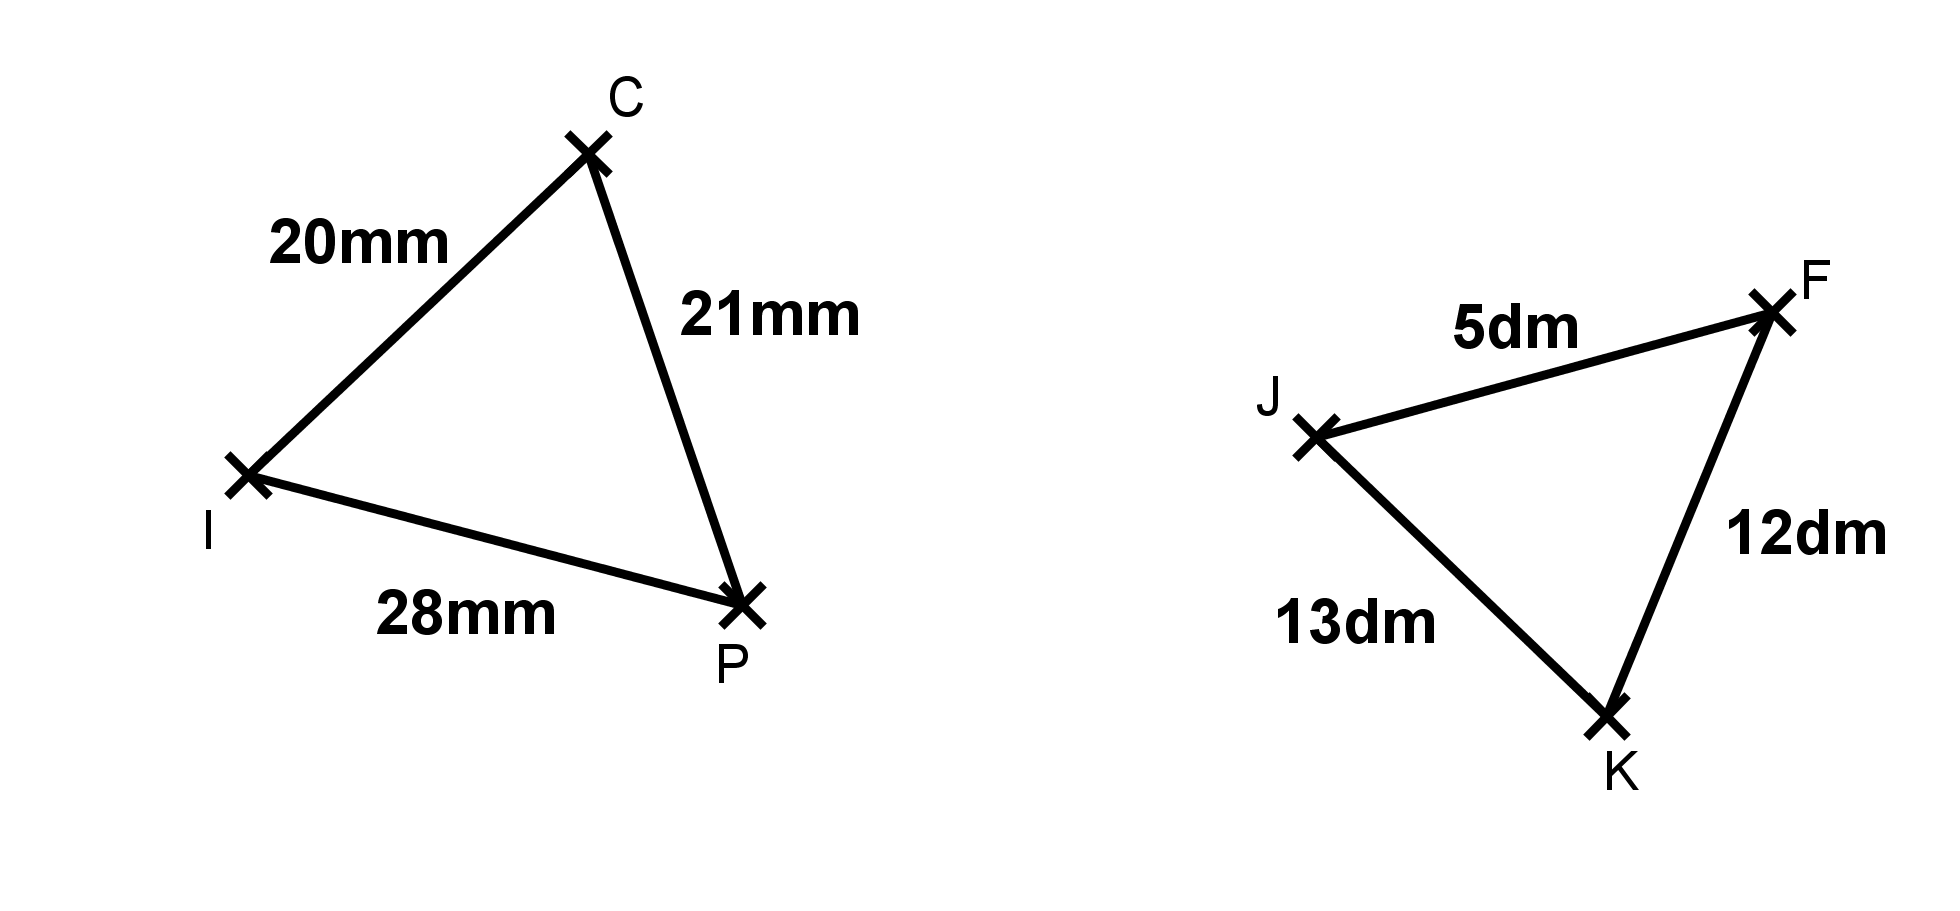
\includegraphics[width=8cm]{images/tri1.png} 
\end{center}

\subsection*{Exercice 3}

\begin{enumerate}
  \item Tracer un segment [AB] de longueur 7cm. Tracer le cercle de diam�tre
  [AB] puis placer sur ce cercle le point C tel que BC=4,5cm.
  \item Que peut-on dire du triangle ABC? Justifier votre r�ponse.
  \item Calculer la longueur AC au millim�tre pr�s.
\end{enumerate}

\subsection*{Exercice 4}


Un arbre s'est bris� en deux en tombant sur un mur de 2,5m de haut. Le pied de
l'arbre est situ� � 4m du pied du mur et la cime de l'arbre s'est retrouv� � 6m
du mur.

On cherche la hauteur totale de l'arbre.

\begin{tabular}{cc}
\begin{minipage}{10cm}
\begin{enumerate}
  \item Faire un sch�ma  en nommant les diff�rents points.
  \item Calculer la hauteur de l'arbre.
  \end{enumerate}
\end{minipage}
&
\begin{minipage}{8cm}
\qquad \qquad 
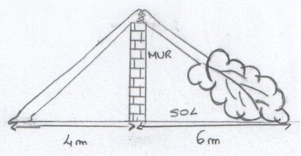
\includegraphics[width=5cm]{images/arbre.jpg}
\end{minipage}
\end{tabular}


  




\subsection*{Exercice 5}


Elodie encadre un tableau (rectangulaire). Pour cela, elle veut d�couper un
morceau de verre rectangulaire. Le morceau d�coup� mesure 36cm et 48cm de c�t�
et 59cm de diagonale. Elodie a-t-elle bien r�ussi sa d�coupe? (commencer par faire un sch�ma du morceau
de verre.)


\subsection*{Exercice 6}

Une lampe co�te 40 \euro. Pendant les soldes, le commer�ant baisse son prix de
25 \%. Quelques jours plus tard, il d�cide de l' augmenter de 20 \%. Quel est
le prix final de la lampe?

\end{document}
